\documentclass{standalone}
\usepackage{tikz}
\usetikzlibrary{decorations.pathreplacing}

\begin{document}

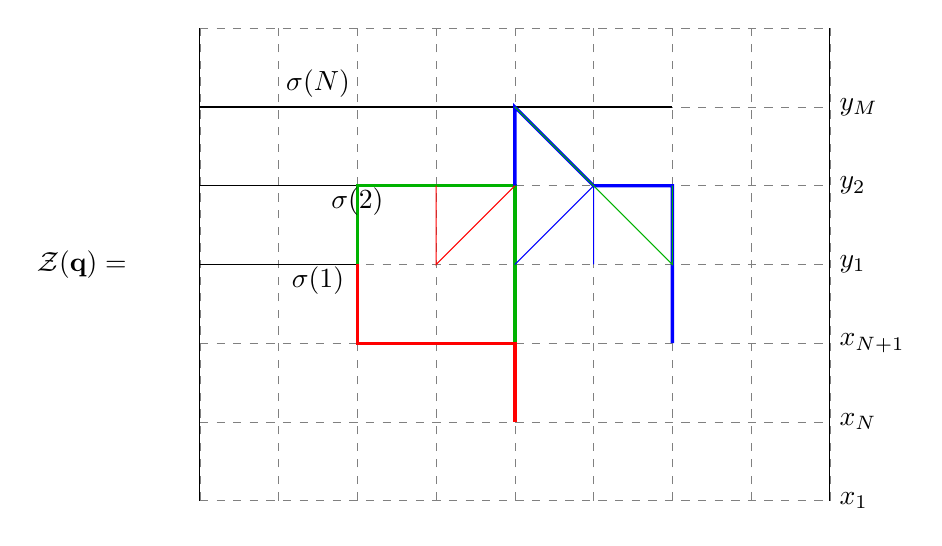
\begin{tikzpicture}
    % Grid lines
    \draw[help lines, dashed] (0,0) grid (8,6);
    
    % Left boundary
    \draw (0,0) -- (0,6);
    
    % Right boundary
    \draw (8,0) -- (8,6);
    
    % Labels on the right boundary
    \node[right] at (8,0) {$x_1$};
    \node[right] at (8,1) {$x_N$};
    \node[right] at (8,2) {$x_{N+1}$};
    \node[right] at (8,3) {$y_1$};
    \node[right] at (8,4) {$y_2$};
    \node[right] at (8,5) {$y_M$};
    
    % Vertical lines at positions M, N and M+N
    \draw (0,3) -- (2,3); % M
    \draw (0,4) -- (4,4); % N
    \draw (0,5) -- (6,5); % M+N
    
    % Lines representing σ(N), σ(2), σ(1)
    \draw[very thick, green!70!black] (2,3) -- ++(0,1) -- ++(2,0) -- ++(0,-3);
    \draw[very thick, blue] (4,4) -- ++(0,1) -- ++(1,-1) -- ++(1,0) -- ++(0,-2);
    \draw[very thick, red] (2,3) -- ++(0,-1) -- ++(2,0) -- ++(0,-1);
    
    % Additional lines for the crossing pattern
    \draw[blue] (5,3) -- ++(0,1) -- ++(-1,-1);
    \draw[red] (3,4) -- ++(0,-1) -- ++(1,1);
    \draw[green!70!black] (6,4) -- ++(0,-1) -- ++(-2,2);
    
    % Labels for the lines on the left
    \node[above] at (1.5,5) {$\sigma(N)$};
    \node[above] at (2,3.5) {$\sigma(2)$}; % Approximated position for the middle line
    \node[above] at (1.5,2.5) {$\sigma(1)$};
    
    % Label for the operator Z(q)
    \node at (-1.5,3) {$\mathcal{Z}(\mathbf{q}) =$};
\end{tikzpicture}

\end{document}